% IMPOSTAZIONI DOCUMENTO 

\documentclass[a4paper, english]{article}

\usepackage[citestyle=numeric,bibstyle=numeric,maxcitenames=1,useprefix,hyperref,natbib,backend=bibtex]{biblatex}
\usepackage[utf8]{inputenc}
\usepackage{babel}
\usepackage{uniudtesi}
\usepackage[nottoc]{tocbibind}
\usepackage{indentfirst}
\usepackage[counterclockwise]{rotating}
\usepackage{listings}
\usepackage{fancyhdr}
\usepackage{enumerate}
\usepackage{longtable}
\usepackage{subcaption}
\usepackage{multirow}
\usepackage{csquotes}
\usepackage{booktabs}
\usepackage{quoting}
\usepackage{listings}
\usepackage{amsmath}
\usepackage{adjustbox}
\usepackage{array}
\usepackage{amsmath,amsfonts,amssymb,amsthm}
\usepackage{latexsym}
\usepackage{caption}
\usepackage{changepage}
\usepackage{enumitem}
\usepackage{threeparttable}
\usepackage{fancyvrb}
\usepackage{makecell}
\usepackage{tocloft}
\usepackage{xstring}
\usepackage{mathtools}
\usepackage{etoolbox}
\usepackage{xcolor,colortbl}
\usepackage{algorithm}
\usepackage{algpseudocode}
\usepackage{hyperref}
\usepackage{titlesec}
\usepackage{xspace}

% NOME DEL FILE CONTENENTE LA BIBLIOGRAFIA. IL FILE DEVE TROVARSI NELLA ROOT DEL FILE .TEX, AVERE IL NOME INDICATO TRA LE PARENTESI GRAFFE ED ESTENSIONE .bib 

\bibliography{bibliography}

% PATH RELATIVO DALLA ROOT DEL FILE TEX ALLA CARTELLA CONTENENTE LE IMMAGINI

\graphicspath{{./immagini/}}

\raggedbottom

% IMPOSTAZIONI FONT 

\renewcommand{\baselinestretch}{1.2}

% OPZIONE CHE CONSENTE DI SPEZZARE LE URL IN QUALUNQUE LORO PUNTO

\expandafter\def\expandafter\UrlBreaks\expandafter{\UrlBreaks
\do\a\do\b\do\c\do\d\do\e\do\f\do\g\do\h\do\i\do\j
\do\k\do\l\do\m\do\n\do\o\do\p\do\q\do\r\do\s\do\t
\do\u\do\v\do\w\do\x\do\y\do\z\do\A\do\B\do\C\do\D
\do\E\do\F\do\G\do\H\do\I\do\J\do\K\do\L\do\M\do\N
\do\O\do\P\do\Q\do\R\do\S\do\T\do\U\do\V\do\W\do\X
\do\Y\do\Z}

% COLONNE TABELLA DIMENSIONE FISSATA 

\newcolumntype{L}[1]{>{\raggedright\let\newline\\\arraybackslash\hspace{0pt}}m{#1}}
\newcolumntype{C}[1]{>{\centering\let\newline\\\arraybackslash\hspace{0pt}}m{#1}}
\newcolumntype{R}[1]{>{\raggedleft\let\newline\\\arraybackslash\hspace{0pt}}m{#1}}

% NO VIRGOLETTE IN BIBLIOGRAFIA

\DeclareFieldFormat[inbook]{title}{#1} 
\DeclareFieldFormat[inproceedings]{title}{#1} 
\DeclareFieldFormat[article]{title}{#1}

% DEFINIZIONE DI MACRO

\newcommand{\N}{\mathbb{N}}

% LSTLISTINGS CON LINE WRAPPING

\lstset{
basicstyle=\small\ttfamily,
columns=flexible,
breaklines=true
}

% VISUALIZZAZIONE DI FILE JSON

\colorlet{punct}{red!60!black}
\definecolor{background}{HTML}{EEEEEE}
\definecolor{delim}{RGB}{20,105,176}
\colorlet{numb}{magenta!60!black}


\lstdefinelanguage{json}{
    basicstyle=\normalfont\ttfamily,
    numbers=left,
    numberstyle=\scriptsize,
    stepnumber=1,
    numbersep=8pt,
    showstringspaces=false,
    breaklines=true,
    frame=lines,
    backgroundcolor=\color{background},
    literate=
     *{0}{{{\color{numb}0}}}{1}
      {1}{{{\color{numb}1}}}{1}
      {2}{{{\color{numb}2}}}{1}
      {3}{{{\color{numb}3}}}{1}
      {4}{{{\color{numb}4}}}{1}
      {5}{{{\color{numb}5}}}{1}
      {6}{{{\color{numb}6}}}{1}
      {7}{{{\color{numb}7}}}{1}
      {8}{{{\color{numb}8}}}{1}
      {9}{{{\color{numb}9}}}{1}
      {:}{{{\color{punct}{:}}}}{1}
      {,}{{{\color{punct}{,}}}}{1}
      {\{}{{{\color{delim}{\{}}}}{1}
      {\}}{{{\color{delim}{\}}}}}{1}
      {[}{{{\color{delim}{[}}}}{1}
      {]}{{{\color{delim}{]}}}}{1},
}

\makeatletter
\renewcommand{\ALG@name}{Listing}
\renewcommand{\listalgorithmname}{List of Listings}
\makeatother

\titleclass{\subsubsubsection}{straight}[\subsection]

\newcounter{subsubsubsection}[subsubsection]
\renewcommand\thesubsubsubsection{\thesubsubsection.\arabic{subsubsubsection}}
\renewcommand\theparagraph{\thesubsubsubsection.\arabic{paragraph}} % optional; useful if paragraphs are to be numbered

\titleformat{\subsubsubsection}
  {\normalfont\normalsize\bfseries}{\thesubsubsubsection}{1em}{}
\titlespacing*{\subsubsubsection}
{0pt}{3.25ex plus 1ex minus .2ex}{1.5ex plus .2ex}

\makeatletter
\renewcommand\paragraph{\@startsection{paragraph}{5}{\z@}%
  {3.25ex \@plus1ex \@minus.2ex}%
  {-1em}%
  {\normalfont\normalsize\bfseries}}
\renewcommand\subparagraph{\@startsection{subparagraph}{6}{\parindent}%
  {3.25ex \@plus1ex \@minus .2ex}%
  {-1em}%
  {\normalfont\normalsize\bfseries}}
\def\toclevel@subsubsubsection{4}
\def\toclevel@paragraph{5}
\def\toclevel@paragraph{6}
\def\l@subsubsubsection{\@dottedtocline{4}{7em}{4em}}
\def\l@paragraph{\@dottedtocline{5}{10em}{5em}}
\def\l@subparagraph{\@dottedtocline{6}{14em}{6em}}
\makeatother

\setcounter{secnumdepth}{4}
\setcounter{tocdepth}{4}

\newcommand{\rsserver}{RS\_Server\xspace}
\newcommand{\rspdf}{RS\_PDF\xspace}
\newcommand{\rsrate}{RS\_Rate\xspace}
\newcommand{\rspy}{RS\_Py\xspace}

\lstset{
columns=flexible,
breaklines=true
}

% INFORMAZIONI GENERALI

\titolo{Readersourcing 2.0:\\ Documentation}
\nomeprogetto{MICHAEL SOPRANO AND STEFANO MIZZARO}

\begin{document}

\maketitle

\tableofcontents

\newpage

\listoffigures

\newpage

\listoftables

\newpage


\section{Introduction}


The Readersourcing 2.0 ecosystem has been built within a research project co-funded by SISSA Medialab\footnote{\url{https://medialab.sissa.it/}} and University of Udine.\footnote{\url{https://www.uniud.it/}} It has been presented by \citet{Soprano2019} during the IRCDL 2019 Conference.\footnote{\url{https://ircdl2019.isti.cnr.it/}} The paper can be found also on Zenodo.\footnote{\url{https://zenodo.org/record/1446468}} The code and the related documentation is available on GitHub.\footnote{\url{https://github.com/Miccighel/Readersourcing-2.0}}

Initially, a recap of its general architecture is presented, followed by a brief description of the role and purpose of each of its components. Specific aspects, such as the technology used, the internal architecture, and the structure of the database, are also discussed. This is achieved through the use of different types of diagrams adhering to the UML standard (unless otherwise specified), which are drawn according to the style rules for that standard proposed by \citet{Fowler03}.

\section{General Architecture}

Readersourcing 2.0 is an ecosystem composed of more than one component. Specifically, it includes \rsserver \cite{RS-Server} (presented in Section~\ref{rs-server}), which acts as a server to gather all the ratings given by readers, and \rsrate \cite{RS-Rate} (presented in Section~\ref{rs-rate}), which acts as a client, enabling readers to rate publications. Although all operations can be carried out directly on the web interface provided by \rsserver, another component, \rspdf \cite{RS-PDF} (presented in Section~\ref{rs-pdf}), is responsible for annotating PDF files using a dedicated software library. This component is utilized by the server-side application. Additionally, \rspy (presented in Section~\ref{rs-py}) provides a fully functional implementation of the RSM and TRM models described by \citet{Soprano2019}. 

Figure~\ref{fig:architecture} provides an overview of the architecture of Readersourcing 2.0, and in the following, we briefly describe these four components. We summarize the capabilities of the ecosystem in Section~\ref{overview}.

\begin{figure}[h]
\centering
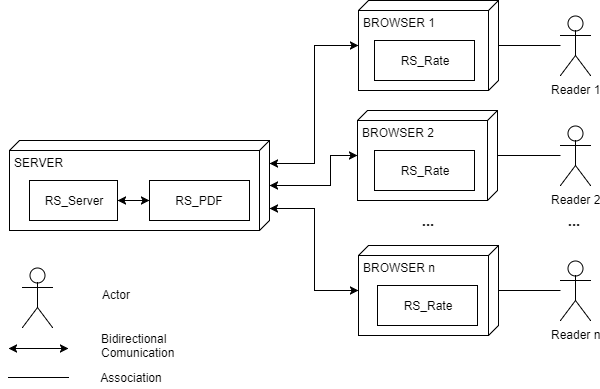
\includegraphics[width=\textwidth]{figures/architecture.png}
\caption{Architecture of Readersourcing 2.0 (NOT UML).}
\label{fig:architecture}
\end{figure}

\section{\rsserver}

\label{rs-server}

\rsserver \cite{RS-Server} is the server-side component that has the task of collecting and aggregating the ratings given by readers and using the RSM and TRM models described by \citet{Soprano2019} in order to compute quality scores for readers and publications. An instance of \rsserver is deployed along one of \rspdf. 
Then, there are up to \emph{n} different browsers along with their end-users, which communicate with the server: each of them is characterized by an instance of \rsrate. Both \rspdf and \rsrate are described in the following.

This setup facilitates interactions between readers and the server through clients installed on readers' browsers or by utilizing the stand-alone web interface provided by \rsserver. These clients are responsible for managing the registration and authentication of readers, handling rating actions, and managing the download actions of link-annotated publications.

During the design phase of \rsserver, strategies were adopted to ensure extensibility and generality. This includes: 
\begin{enumerate}[label=(\roman*)]
\item Straightforward addition of new models. 
\item A shared input data format among all models.
\item A standard procedure for models needing to save values locally in the \rsserver database.
\end{enumerate}

\subsection{Implementation and Technology}

\rsserver is developed in Ruby on Rails,\footnote{\url{https://rubyonrails.org/}} which is a framework that allows building applications strongly based on the Model-View-Controller (MVC) architectural pattern. The technology used to develop \rsserver is an open-source web application framework called \emph{Ruby on Rails} (also referred to as \emph{RoR} or \emph{Rails} only). More specifically, \emph{Rails} is the framework built above \emph{Ruby}, the actual programming language. It allows building applications strongly based on the Model-View-Controller (MVC) architectural pattern.

The MVC pattern allows for the separation of the control logic of the program from data presentation and business logic. Therefore, it facilitates the creation of an effective architecture from the initial design phase. Figure \ref{fig:mvc} provides an intuitive representation of the structure that this pattern enables. The structure comprises three distinct entities: the \emph{Controller}, responsible for managing control logic; the \emph{Model}, tasked with encapsulating business logic; and the \emph{View}, responsible for implementing data presentation.

\begin{figure}[!tbp]
\centering
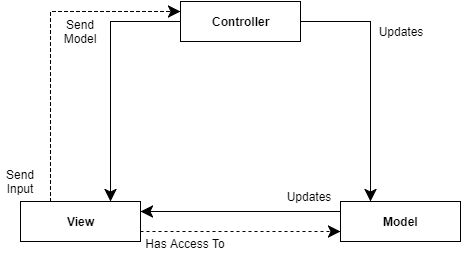
\includegraphics[scale=0.7]{figures/mvc.png}
\caption{Intuitive scheme of the MVC pattern (NOT UML).}
\label{fig:mvc}
\end{figure}

The Controller has direct access to both the Model and the View. Typically, it receives user input from the View and, based on this input, updates the internal state of the Model using its methods. Subsequently, the Controller sends the updated Model to the View, which then utilizes this information to obtain and display the results of the processing. In a generic software system, there can be more than one Controller, and each Controller may manage multiple instances of the Model. In MVC frameworks designed for web applications, such as Rails, it is common practice to have a number of Controllers equal to the entities modeled within the application domain. Additionally, there may be more than one View implementation to present the internal state of a specific type of Model.

The use of the MVC pattern is not the sole foundational principle of Rails. One of the most crucial principles shaping Rails for the development of high-quality applications is \lq\lq Convention Over Configuration\rq\rq{}. In essence, the framework aims to reduce the decisions developers need to make during application construction by embracing standard conventions that can be modified for increased flexibility if necessary. To delve deeper into the foundational principles of Rails, one can refer to the \lq\lq Rails Doctrine\rq\rq{}.\footnote{\url{https://rubyonrails.org/doctrine/}}

As a final note, Rails is a dynamically evolving framework widely employed in the industry by prominent players such as \emph{GitHub}, \emph{SoundCloud}, and others. It is a widely embraced and esteemed technology with an active community and abundant learning resources.

\subsection{Communication Paradigm}

A modern MVC framework like Rails provides the capability to develop various types of web applications. One such possibility is the creation of a \emph{Web Service}, which is a software component capable of executing various operations made remotely accessible through the exchange of messages encoded in a standard interchange format such as \emph{JSON}. This is facilitated by a transport layer built on top of basic Internet protocols like \emph{HTTP}. However, the implementation of this functionality must adhere to a paradigm that precisely defines the available functionalities (resources and operations) and specifies the required messages for accessing them.

One of the communication paradigms for Web Services is \emph{RESTful} (\emph{REpresentational State Transfer}). In this paradigm, the functionalities of a Web Service are represented by resources identified through different URIs, and the type of HTTP message sent determines the operation to be performed. The result of the operation initiated by the received message from the Web Service is a new message encoded in the same interchange format as the one sent. It is the client's responsibility to accurately interpret and utilize the response from the Web Service.

\rsserver is a Web Service (Server API-Only in Rails terminology) following a communication paradigm based on RESTful interfaces. It operates through the exchange of messages encoded in JSON format, utilizing the transport layer provided by the HTTP protocol.

The communication interface of \rsserver is continuously evolving. Given the dynamic nature of its development, providing a comprehensive inclusion in this document is impractical. However, interested parties can freely explore the evolving interface, including examples of requests, by visiting the following URL.

\begin{table}[h]
\centering
\begin{tabular}{p{12cm}}
  \toprule
	\url{https://documenter.getpostman.com/view/4632696/RWTiwfV4?version=latest}  \\
 \toprule
  \end{tabular}
\end{table}

To illustrate, Table \ref{tab:rest} presents a subset of the RESTful interface of \rsserver. These operations encompass all functionalities related to managing one of the entities within the application domain, specifically, publications. Suppose a user initiates a ``show'' operation for a publication with an identifier equal to 1 by accessing the corresponding endpoint. In response, \rsserver would provide a JSON-encoded response similar to the example below.

\begin{lstlisting}[language=json,firstnumber=1]
{
  "id": 1,
  "doi": "10.1140/epjc/s10052-018-6047-y",
  "title": "Uncertainties in WIMP dark matter scattering revisited",
  "author": "John Ellis",
  "creator": "Springer",
  "producer": null,
  "...": ...,
  "created_at": "2018-08-02T13:27:46.988Z",
  "updated_at": "2018-08-02T13:27:49.135Z",
  "...": ...,
}
\end{lstlisting}

\begin{table}
\centering
\begin{threeparttable}
\begin{tabular}{p{5.2cm}C{1.5cm}C{2cm}p{5cm}}
\toprule
\textbf{Endpoint}  &\textbf{HTTP Message} & \textbf{Operation} & \textbf{Description} \\
\midrule
/publications.json & GET & Index & Fetches the entire collection of Publications. \\
\midrule
/publications/list & GET & List & Fetches the entire collection of Publications (server-side view). \\
\midrule
/publications/1.json & GET & Show & Returns the Publication with identifier equal to 1.\\
\midrule
/publications/lookup.json & POST & Lookup & Searches for a Publication; if it doesn't exists, it is fetched from the given URL. \\
\midrule
/publications/random.json & GET & Random & Returns a random Publication. \\ 
\midrule
/publications/1/is\_rated.json & GET & Is Rated & Checks if the Publication with identifier equal to 1 has been rated by at least one reader. \\
\midrule
/publications/1/is\_saved\_for\_later.json & GET & Is Saved For Later & Checks if the Publication with identifier equal to 1 has been saved for later by the current user. \\
\midrule
/publications.json & POST & Create & Creates a new Publication. \\
\midrule
/publications/is\_fetchable.json & POST & Is Fetchable & Checks if the provided URL contains a fetchable Publication. \\
\midrule
/publications/extract.json & POST & Extract & Extract the rating url from a link-annotated Publication. \\
\midrule
/publications/fetch.json & POST & Fetch & Fetches a Publication from the given URL. \\
\midrule
/publications/1/refresh.json & GET & Refresh & Fetches again the Publication with identifier equal to 1. \\
\midrule
/publications/1.json & PUT & Update & Updates the Publication with identifier equal to 1. \\
\midrule
/publications/1.json & DELETE & Delete & Deletes the Publication with identifier equal to 1.\\
\midrule
\dots & \dots & \dots & \dots \\
\bottomrule
\end{tabular}
\caption{Subset of the RESTFul interface of \rsserver.}
\label{tab:rest}
 \end{threeparttable}
\end{table}

\subsection{Database}

To facilitate the implementation of functionalities such as the storage of link-annotated publications and user authentication, a database schema has been defined, as illustrated in Figure~\ref{fig:er}. Within the application domain of Readersourcing 2.0, three main entities have been modeled:

\begin{itemize}
\item \textbf{Users}: models the users of the system, characterized by their personal data. Users may have an optional \emph{ORCID} and a boolean indicating whether they wish to receive emails. Additionally, various attributes are utilized to store different types of tokens, enabling operations such as password reset.
\item \textbf{Ratings}: represents the ratings provided by readers for publications. These ratings are characterized by a numerical score. The entity also includes a boolean to indicate whether a rating is anonymous, and another boolean to track whether it has been edited at a later time.
\item \textbf{Publications}: models the publications that have been rated by readers. These publications are characterized by an optional \emph{DOI}, various metadata, and a set of attributes used to manage server filesystem paths. These attributes ensure the storage of both the original and link-annotated files, both encoded in PDF format.
\end{itemize}
In addition, each of these entities is further characterized by additional attributes (\emph{steadiness}, \emph{informativeness}, \dots), representing the scores or parameters computed by the Readersourcing models.

\begin{figure}[!tbp]
\centering
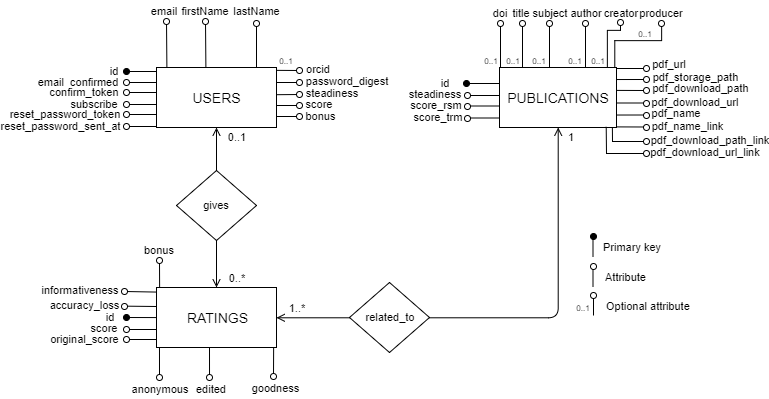
\includegraphics[width=\textwidth]{figures/er.png}
\caption{Entity-Relationship schema of the \rsserver database (NOT UML).}
\label{fig:er}
\end{figure}

Figure~\ref{fig:er} also depicts two relationships (\emph{gives} and \emph{related\_to}) that exist between these three entities. These relationships facilitate the ``tying together'' of the entities they reference and ensure compliance with the \emph{referential integrity} constraint.

In particular, the \emph{gives} relation establishes that a user can give $[0,\dots ,n]$ different ratings, with the constraint that a single rating can be expressed at most by a user. The multiplicity equal to $0$ regarding users in Figure~\ref{fig:er} may seem unusual at first glance. However, this constraint is intended to allow the expression of anonymous ratings.

Similarly, the \emph{related\_to} relation establishes that a rating is associated with a specific publication, while a publication can be characterized by $[1,\dots ,n]$ different ratings. This structure naturally accommodates other constraints, such as the condition that if at least one publication does not exist, no ratings need to exist.

\subsection{Class Diagram}

Figure~\ref{fig:class-1} shows a diagram of the main classes of \rsserver. As one can see, the convention for which there is an MVC triple for each of the entities modeled in the application domain is followed, althought Views are not shown in the diagram because in this case they are just simple methods. The Controller methods represent actions that a user can perform on individual entities or on collections of them, thus mapping the endpoints of the communication protocol used in order to allow the communication between \rsserver and the instances of \rsrate. As for the Models, their attributes represent the characteristics of the reference entity, while their methods encapsulate the business logic.

\begin{figure}[!tbp]
\centering
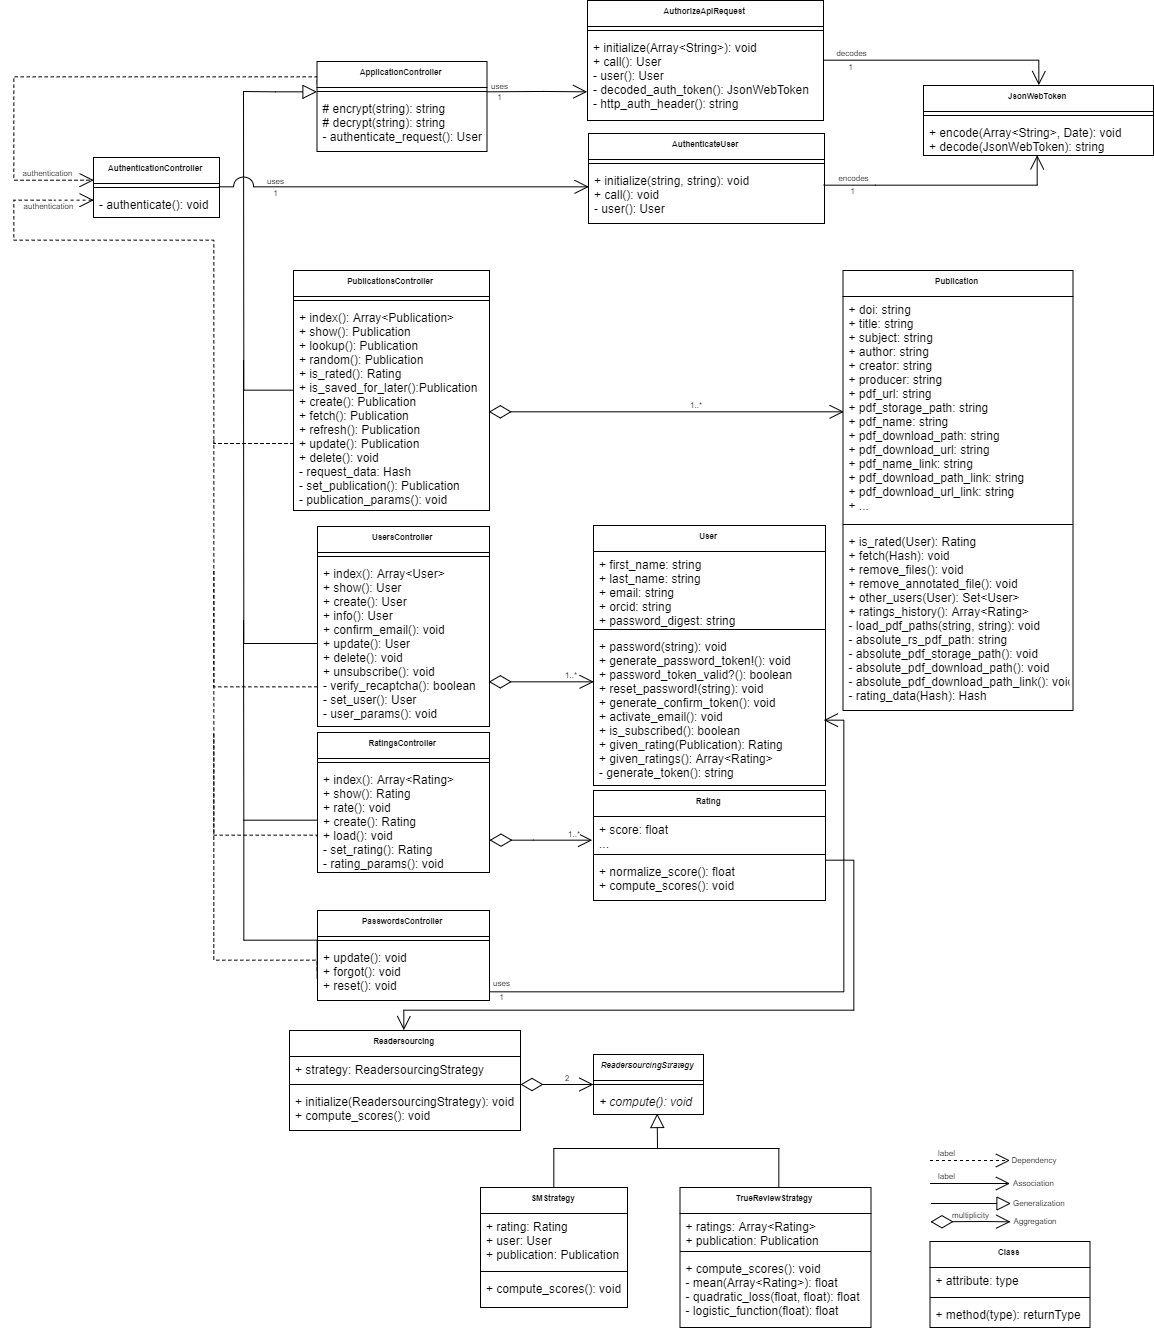
\includegraphics[scale=0.4]{figures/classi-1.png}
\caption{Class diagram of \rsserver.}
\label{fig:class-1}
\end{figure}

Additionally, there are two controllers—namely, the \emph{Application Controller} and the \emph{Authentication Controller}—tasked with managing user authentication. As mentioned earlier, \rsserver functions as a Web Service. In this setup, the user interface is presented directly on instances of \rsrate. Consequently, these instances send messages to which \rsserver responds once the necessary processing is complete, following the RESTful communication paradigm.

Due to this design choice, the traditional server-side approach to user authentication, where information about the logged user is stored in session data, is not viable. This is because the RESTful paradigm is \emph{stateless}. To authenticate themselves, users must attach a \emph{token} to each request, identifying their validity within the system. Therefore, a \emph{token-based} authentication approach has been implemented.

When a user initiates the first request to \rsserver after a period of inactivity, they are required to fill in the login form. If the provided credentials exist in the database, they are encrypted to form a \emph{payload}. This payload, combined with a unique \emph{signature}, results in an alphanumeric JSON string—the actual token. The generated token is then sent to the user's \rsrate instance, which securely stores it in a cookie with an expiration date. Subsequent requests to \rsserver from the \rsrate instance include the previously obtained token in the \emph{Authorization} header of the HTTP payload, demonstrating that the user has successfully completed the authentication procedure.

For \rsserver, upon receiving a request, if a token is present, it is extracted and decoded. If the decoded token corresponds to one saved in the database, the user identified by the payload is authorized to proceed. Figure~\ref{fig:auth} provides an intuitive illustration of this authentication process.

\begin{figure}[!tbp]
\centering
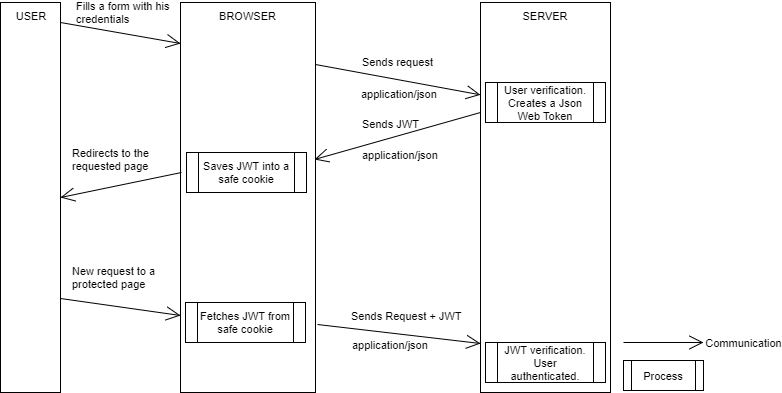
\includegraphics[width=\textwidth]{figures/autenticazione.png}
\caption{Representation of the token-based authentication process (NOT UML).}
\label{fig:auth}
\end{figure}

Additionally, there is another set of classes serving purposes beyond representing MVC triples for the entities in the application domain. Specifically, these classes are internally utilized by the model containing the business logic to manage given ratings and are responsible for implementing the Readersourcing models. The structure of these classes adheres to a design pattern known as \emph{Strategy} (specifically, \emph{Readersourcing}, \emph{ReadersourcingStrategy}, \emph{RSMStrategy}, and \emph{TRMStrategy}). The use of the \emph{Strategy} pattern allows for the integration of new models at a later time without necessitating radical changes to the structure of \rsserver.

\subsection{Deploy}

There are three main modalities that can be used to deploy a working instance of \rsserver in the \emph{development} or \emph{production} environment. The former environment must be used if there is the need to:
\begin{itemize}
\item add custom \emph{Readersourcing}-based models;
\item extend/modify the current implementation of \rsserver;
\item simply to test it in a safe way.
\end{itemize}

In the following, three deployment modalities to obtain a working instance of \rsserver are described along with their requirements. The first two modalities allow for starting \rsserver on the local machine, enabling the editing of its source code, and building a Docker image that can be deployed via local containers in a production-ready environment. The third modality enables deploying \rsserver as a Heroku application.

It is strongly suggested to read the section dedicated to the environment variables (Section \ref{env-vars}), as \rsserver will not function properly without them.

\subsubsection{Modality 1: Manual}

\label{deploy1}

This modality allows for manually downloading and initializing \rsserver's codebase on a local machine. It is the most demanding in terms of prerequisites, as it assumes having a full and working installation of \emph{Ruby}, \emph{JDK} (Java Development Kit), and \emph{PostgreSQL}. Despite these requirements, it offers greater flexibility.

\subsubsubsection{Requirements}

\begin{itemize}
\item Ruby $==$ 2.7.8;
\item JDK (Java Development Kit) $==$ 11.0.19;
\item PostgreSQL $>=$ 11.2.
\end{itemize}

\subsubsubsection{How To}

Clone the \rsserver repository,\footnote{\url{https://github.com/Miccighel/Readersourcing-2.0-RS_Server}} and navigate to its main directory using a command line prompt (you should see \verb|app|, \verb|bin|, \verb|config|, etc., folders with an \verb|ls| or \verb|dir| command), then type \verb|gem install bundler|. This gem (dependency) provides a consistent environment for Ruby projects, like \rsserver, by tracking and installing the exact gems (dependencies) and versions needed.

To fetch all dependencies required by \rsserver, type \verb|bundle install| and wait for the process to complete.

The next two commands are necessary \emph{only before the first startup of \rsserver} because they will create and set up the database. Ensure that the PostgreSQL service is started and ready to accept connections on port 5432. Type \verb|rails db:create| to create the database and \verb|rails db:migrate| to create the required tables.

Now, create a \verb|.env| file as explained in Section~\ref{set-var} and set the required environment variables.

Optionally, you can type \verb|rails db:seed| to seed some sample data into the database. After these commands, everything is ready to launch \rsserver in \emph{development} or \emph{production} mode. To do that, type \verb|cd bin| to move inside the \verb|bin| directory, and then type
\begin{verbatim}
rails server -b 127.0.0.1 -p 3000 -e development
\end{verbatim}
with the proper values for \verb|-b|, \verb|-p|, and \verb|-e| options. If the sample values are used, \rsserver will be started and bound to the \verb|127.0.0.1| IP address with port \verb|3000| and the \verb|development| environment. Every HTTP request, therefore, must be sent to the \verb|http://127.0.0.1:3000| address.

\subsubsubsection{Quick Cheatsheet}

\begin{enumerate}
\item \verb|cd| to main directory;
\item \verb|gem install bundler|;
\item \verb|bundle install|;
\item \verb|rails db:create|;
\item \verb|rails db:migrate|;
\item create and populate the \verb|.env| file;
\item \verb|cd bin|;
\item \verb|rails server -b <your_ip_address> -p <your_port> -e development| or\\ \verb|rails server -b <your_ip_address> -p <your_port> -e production|.
\end{enumerate}

\subsubsection{Modality 2: Manual Way (Using Docker)}

This modality allows you to download and initialize \rsserver's codebase on a local machine using a faster and less frustrating approach based on Docker, despite being less flexible. Docker is a project that automates the deployment phase by distributing an \emph{image} of an application inside a \emph{container}.

An \emph{image} is a lightweight, standalone, and executable package of software that includes everything needed to run an application: code, runtime, tools, libraries, and settings. This means that there is no need to manually install the runtimes, libraries, or dependencies needed to run an application since the Docker Engine will automatically initialize everything.

A \emph{container} is a standard unit of software that packages up code and all its dependencies so the application runs quickly and reliably from one computing environment to another. Only a working installation of \verb|Docker Desktop CE (Community Edition)| is required.

\subsubsubsection{Requirements}

\begin{itemize}
\item Docker Desktop CE (Community Edition);\footnote{\url{https://www.docker.com/products/docker-desktop}}
\end{itemize}

\subsubsubsection{How To}

Clone \rsserver repository\footnote{\url{https://github.com/Miccighel/Readersourcing-2.0-RS_Server}} and navigate to its main directory using a command line prompt. Now, type \verb|ls| or \verb|dir|. You should see a \verb|docker-compose.yml| file and a \verb|Dockerfile|. If you do not see them, please make sure you are in the main directory of the cloned repository.

Before proceeding, \emph{ensure that your Docker Engine is running}. Otherwise, the following commands will not work. At this point, two different scenarios can unfold.

\paragraph{Scenario 1: Deploy With Remote Images}

If there is no need to edit the source code of \rsserver, the Docker Engine can fetch the dependencies required in the \verb|docker-compose.yml| file and initialize the application. The dependencies specified in the file are an image of PostgreSQL for the database and one of \rsserver itself, released on the Docker Hub.\footnote{\url{https://cloud.docker.com/repository/docker/miccighel/rs_server}}

To do this, open the \verb|docker-compose.yml| file and uncomment the following section and, additionally, comment out the remaining lines of code in the file.
\begin{verbatim}
----------- SCENARIO 1: DEPLOY WITH REMOTE IMAGES ----------
----------- END OF SCENARIO 1: DEPLOY WITH REMOTE IMAGES ----------
\end{verbatim} 

Next, from the command line prompt, type \verb|docker-compose up| and wait for the process to finish. Note that it may take several minutes. 
Once the Docker Engine completes the process, a container with a working instance of \rsserver will be started.

Optionally, you can type \verb|docker-compose run rails db:seed| to seed some sample data in the database. \rsserver will be started and bound 
to the \verb|0.0.0.0| IP address with port \verb|3000| and the \verb|production| environment. Every HTTP request, therefore, must be sent to 
the \verb|http://0.0.0.0:3000| address.

As can be seen, there is no need to manually start the server by specifying its IP address, port, and environment, or to create and migrate 
the database. The Docker Engine will perform that automatically. If you want to set a custom IP address or port or switch 
to the production environment, edit the \verb|command| key inside the \verb|docker-compose.yml| file.

To stop the container, simply type \verb|docker-compose down|.

\paragraph{Scenario 2: Deploy With Local Build}

If the source code of \rsserver has been edited, the application must be built from scratch by the Docker Engine according to the structure 
specified in the \verb|Dockerfile|. After the image build phase, the Docker Engine can fetch the required dependencies outlined in 
the \verb|docker-compose.yml| file and initialize \rsserver, as in the previous scenario.

To do this, open the \verb|docker-compose.yml| file and uncomment the following section. 
Additionally, comment out the remaining lines of code in the file.
\begin{verbatim}
----------- SCENARIO 2: DEPLOY WITH LOCAL BUILD ----------
----------- END OF SCENARIO 2: DEPLOY WITH LOCAL BUILD -----------
\end{verbatim} 

Next, from the command line prompt, type \verb|docker-compose up| and wait for the process to finish. Note that it may take several minutes. 
Once the Docker Engine completes the process, a container with a working instance of \rsserver will be started and bound to the \verb|0.0.0.0| 
IP address with port \verb|3000| and the \verb|production| environment. Therefore, every request must be sent to the \verb|http://0.0.0.0:3000| address.

Similar to the previous scenario, there is no need to manually start the server by specifying its IP address, port, and environment or to create and migrate the database. If you want to set a custom IP address or port or switch to the production environment, edit the \verb|command| key inside the \verb|docker-compose.yml| file.

To stop the container, simply type \verb|docker-compose down|.

\paragraph{Quick Cheatsheet}

\begin{itemize}
\item \verb|cd| to main directory;
\item create and populate the \verb|.env| file;
\item \verb|docker-compose up|;
\item \verb|docker-compose run rails db:seed| (optional);
\item \verb|docker-compose down| (to shutdown and undeploy).
\end{itemize}

\subsubsection{Modality 3: Deploy on Heroku}

\label{modality:3}

\emph{Heroku} is a cloud platform-as-a-service (PaaS) that simplifies building, deploying, and scaling web applications and services for developers. This deploy modality enables the use of its container registry for a Docker-based production-ready deployment of \rsserver on the platform, facilitated by the \verb|Heroku Command Line Interface (CLI)|.\footnote{\url{https://devcenter.heroku.com/articles/heroku-cli}} It's important to note that this modality can only be used with the \emph{production} environment of the application.

Regarding the prerequisites for this modality, the developer must create an \verb|app| on Heroku and then provision it with two addons: \emph{PostgreSQL}\footnote{\url{https://elements.heroku.com/addons/heroku-postgresql}} for the database and one for mail-related functionalities, such as \emph{Twilio SendGrid}.\footnote{\url{https://elements.heroku.com/addons/sendgrid}} The Heroku tutorials provide a comprehensive overview 
of the platform. Additionally, a working installation of \verb|Docker Desktop CE (Community Edition)| on the machine used for deployment is required.

\subsubsubsection{Requirements}

\begin{itemize}
\item Heroku account;
\item Heroku application provisioned with:
\begin{itemize}
\item PostgreSQL addon;
\item a mail-related addon such as Twilio SendGrid;
\end{itemize}
\item Heroku CLI;
\item Docker Desktop CE (Community Edition);
\end{itemize}

\subsubsubsection{How To}

Clone \rsserver repository\footnote{\url{https://github.com/Miccighel/Readersourcing-2.0-RS_Server}} and navigate to the main directory using a command line prompt. Now, type \verb|ls| or \verb|dir|. You should see a \verb|Dockerfile|. If not, please ensure you are in the main directory of the cloned repository.

Before proceeding, \emph{make sure that your Docker Engine is running}. Otherwise, the following commands will not work.

Log in using your credentials by typing \verb|heroku login|. Next, log in to the Heroku container registry by typing \verb|heroku container:login|.

To build and upload your instance of \rsserver using Docker, type
\begin{verbatim}
heroku container:push web --app your-app-name
\end{verbatim}
When the process completes, type \verb|heroku container:release web| to make it publicly accessible.

Optionally, you can type \verb|heroku run rails db:seed| to seed some sample data in the database, and \verb|heroku open| to open the browser and be redirected to the homepage of the \verb|<your_app_name>| application.

Similar to the previous modality, there is no need to manually start the server by specifying its IP address, port, and environment, or to create and migrate the database since Heroku (through the Docker Engine) will take care of that for you.

\subsubsubsection{Quick Cheatsheet}

\begin{itemize}
\item \verb|cd| to main directory;
\item \verb|heroku login|;
\item \verb|heroku container:login|;
\item \verb|heroku container:push web --app <your-app-name>|;
\item \verb|heroku container:release web --app your-app-name|;
\item \verb|heroku open --app your-app-name| (optional);
\item set the environment variables on your Heroku app.
\end{itemize}

\subsubsection{Environment Variables}

\label{env-vars}

Regardless of the chosen deployment modality, the developer must provide values for (at least a portion of) the \emph{environment variables}, as they cannot be checked into a repository due to safety reasons. In the following, each of these available variables is described 
along with an explanation of which deployment modality requires their usage.

\begin{longtable}{p{3.5cm}p{3.2cm}p{2.5cm}p{2cm}p{2.7cm}}
\toprule
\textbf{Environment Variable}  &\textbf{Description} & \textbf{Deploy Modality} & \textbf{Environment} & \textbf{Where To Set} \\
\midrule
\endhead
\verb|SECRET_DEV_KEY| & Private key used to encrypt strings in the \verb|development| environment.  & 1 - 2 & \verb|development| & \verb|.env| file \\
\midrule
\verb|SECRET_PROD_KEY| & Private key used to encrypt strings in the \verb|production| environment. & 1 - 2 - 3 & \verb|production| & \verb|.env| file, Heroku App \\
\midrule
\verb|POSTGRES_USER| & Username the admin user of the database & 1 - 2 - 3 & \verb|development|, \verb|production| & \verb|.env| file, Heroku App \\
\midrule
\verb|POSTGRES_PASSWORD| & Password of the admin user of the database & 1 - 2 - 3 & \verb|development|, \verb|production| & \verb|.env| file, Heroku App \\
\midrule
\verb|POSTGRES_DB| & Name of the database & 1 - 2 - 3 & \verb|development|, \verb|production| & \verb|.env| file, Heroku App \\
\midrule
\verb|POSTGRES_HOST| & Hosting address of the database & 1 - 2 - 3 & \verb|development|, \verb|production| & \verb|.env| file, Heroku App \\
\midrule
\verb|DATABASE_URL| & Full connection PostgreSQL connection string of the database. & 1 - 2 - 3 & \verb|development|, \verb|production| & \verb|.env| file, Heroku App \\
\midrule
\verb|SMTP_USERNAME| & Username of the SMTP mail server & 1 - 2 - 3 & \verb|production| & \verb|.env| file, Heroku App \\
\midrule
\verb|SMTP_PASSWORD| & Password of the SMTP mail server & 1 - 2 - 3 & \verb|production| & \verb|.env| file, Heroku App \\
\midrule
\verb|SMTP_DOMAIN_NAME| & Domain of the SMTP mail server & 1 - 2 - 3 & \verb|production| & \verb|.env| file, Heroku App \\
\midrule
\verb|SMTP_DOMAIN_ADDRESS| & Full address of the SMTP mail server & 1 - 2 - 3 & \verb|production| & \verb|.env| file, Heroku App \\
\midrule
\verb|EMAIL_BUG_REPORT| & Email address to receive bug reports & 1 - 2 - 3 & \verb|development|, \verb|production| & \verb|.env| file, Heroku App \\
\midrule
\verb|EMAIL_ADMIN| & Email address to receive general questions & 1 - 2 - 3 & \verb|development|, \verb|production| & \verb|.env| file, Heroku App \\
\midrule
\verb|RAILS_LOG_TO_STD| & When set to \verb|true|, forces the application to write its logs to the standard output. & 1 - 2 - 3 & \verb|production| & \verb|.env| file, Heroku App \\
\bottomrule
\caption{Environment variables of \rsserver.}
\label{env}
\end{longtable}

\subsubsection{Setting Variables}

\label{set-var}

To set an environment variable in a local \verb|.env| file, create it inside the main directory of \rsserver. Then, populate it in a \verb|key=value| fashion.
To set an environment variable in a Heroku app, simply follow the guide.\footnote{\url{https://devcenter.heroku.com/articles/config-vars}} In Heroku terminology, environment variables are called \verb|config vars|.

To provide an example, the following is the content of a valid \verb|.env| file.

\begin{algorithm}[h]
\caption{Content of a valid \texttt{.env} file.}
\label{env-file}
\begin{algorithmic}[1]
\State$\text{SECRET\_PROD\_KEY=your\_secret\_prod\_key\_value}$
\State$\text{DATABASE\_URL=your\_postgresql\_database\_connection\_string}$
\State$\text{SMTP\_USERNAME=your\_smtp\_username}$
\State$\text{SMTP\_PASSWORD=your\_smtp\_password}$
\State$\text{SMTP\_DOMAIN\_NAME=your\_smtp\_domain\_name}$
\State$\text{SMTP\_DOMAIN\_ADDRESS=your\_smtp\_domain\_address}$
\State$\text{EMAIL\_BUG\_REPORT=your\_bug\_report\_mail}$
\State$\text{EMAIL\_ADMIN=your\_contact\_mail}$
\end{algorithmic}
\end{algorithm}

\subsubsection{Sending Mails}

\rsserver supports any SMTP-based mail server to send emails for tasks such as confirming user registration, reporting bugs, or recovering forgotten passwords.

Understanding the values used to populate the \verb|SMTP_| environment variables can sometimes lead to ambiguity. Let's consider the case of the proposed add-on, Twilio Sendgrid,\footnote{\url{https://sendgrid.com/}} both when deploying \rsserver manually and on Heroku.
In the first case, after creating an account, you need to verify a single
sender address or a whole domain using the provided \verb|DNS records|. To integrate the service into an instance of \rsserver deployed anywhere outside Heroku, you must use a supported SMTP configuration.\footnote{\url{https://app.sendgrid.com/guide/integrate/langs/smtp}} Thus, the values of the environment variables must be in this form:
\begin{verbatim}
SMTP_USERNAME: apikey
SMTP_PASSWORD: <your_api_key_value>
SMTP_DOMAIN_NAME: <your_domain_address>
SMTP_DOMAIN_ADDRESS: smtp.sendgrid.net
\end{verbatim}
However, while using the addon provided by Heroku,\footnote{\url{https://elements.heroku.com/addons/sendgrid}} the values provided for the environment variables need to be slightly different:
\begin{verbatim}
SMTP_USERNAME: <your_sendgrid_account_username>
SMTP_PASSWORD: <your_sengrid_password_account>
SMTP_DOMAIN_NAME: <your_domain_address>
SMTP_DOMAIN_ADDRESS: smtp.sendgrid.net
\end{verbatim}

\subsubsection{Connecting To The Database}

A full connection string to a PostgreSQL database provided through the \verb|DATABASE_URL| variable \emph{takes precedence} over each \verb|POSTGRES_| variable. It is thus important to provide the former environment variable or the set of the latter ones. This holds for both the \emph{development} and \emph{production} environments. Indeed, the final connection string is built as such:
\begin{lstlisting}
<%= ENV['DATABASE_URL'] || "postgresql://#{ENV['POSTGRES_USER'] || 'postgres'}:#{ENV['POSTGRES_PASSWORD']}@#{ENV['POSTGRES_HOST'] || 'localhost'}/#{ENV['POSTGRES_DB'] || 'rs_server'}" %>
\end{lstlisting}

\subsubsection{Logging To The Standard Output}

An instance of \rsserver deployed in development writes its logs to the standard output as the default behavior. In a \emph{production} environment, on the other hand, the logs are written in the \verb|logs/production.log| file. Thus, forcing Rails to write logs in the standard output using the \verb|RAILS_LOG_TO_STD| variable can be useful for quick 
debugging purposes when testing the production environment.

\section{\rspdf}

\label{rs-pdf}

\rspdf \cite{RS-PDF} is the software library utilized by \rsserver to edit the PDF files and add the required URL when a reader requests to save a publication for later reading. 

It is characterized by a command-line interface, allowing \rsserver to use it directly. Since they are deployed together, they can communicate without the need for complex channels and paradigms.

\subsection{Implementation and Technology}

The technology used to develop \rspdf is the Kotlin object-oriented programming language, known for its full compatibility with the Java Virtual Machine. This feature is crucial because it allows a developer to leverage code contained in any other software published in JAR format and, more generally, to import any Java class, interacting with them through the syntax of Kotlin itself.

This programming language has been chosen because it incorporates many modern features and receives robust support. Furthermore, it has openings to other platforms, greatly expanding its potential applications. The most significant reason, however, is that the underlying tool used to edit files encoded in PDF format is \emph{PDFBox},\footnote{\url{https://pdfbox.apache.org/}} a software library developed with Java and proposed as a complete toolkit for editing files in that specific format. Therefore, \rspdf serves as a wrapper for PDFBox, adding the necessary links inside the PDFs requested by readers.


Kotlin has been created by JetBrains,\footnote{\url{https://www.jetbrains.com/}} which, in the first half of 2017, signed an agreement with Google to elevate Kotlin to the status of a first-class language for development on the Android platform.\footnote{\url{https://blog.jetbrains.com/kotlin/2017/05/kotlin-on-android-now-official/}} Moreover, in the same year, JetBrains announced the ability to compile programs written in Kotlin directly into machine language, thus avoiding the use of the JVM.

On the web, it is possible to find different pages with comparisons between Kotlin and other languages, including the official one\footnote{\url{https://kotlinlang.org/docs/reference/comparison-to-java.html}} made by JetBrains with Java, and several articles\footnote{\url{https://medium.com/@octskyward/why-kotlin-is-my-next-programming-language-c25c001e26e3}} by developers enthusiastic about this programming language.

\subsection{Package Diagram}

Figure \ref{fig:package} depicts a diagram illustrating the packages in which \rspdf is divided. This diagram offers a high-level overview of the internal architecture of the software, providing valuable insights into its structure.

\begin{figure}[!tbp]
\centering
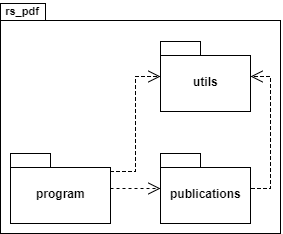
\includegraphics[scale=0.7]{figures/package.png}
\caption{Package diagram of \rspdf.}
\label{fig:package}
\end{figure}

In particular, the interaction with \rsserver takes place within the \textbf{program} package. The server-side component itself can utilize the functionalities of \rspdf by executing it on the JVM with a special set of command-line options. Within this package, the parsing of the values received for each of these options and the management of the execution flow based on these values occur.

The \textbf{utils} package is responsible for providing useful tools to the remaining components of \rspdf. Within this package, shared constants and methods are implemented, enabling access to the logging functionality. As evident from the diagram in Figure~\ref{fig:package}, the other packages depend on it, particularly for some of the values of its constants.

The \textbf{publications} package contains the business logic to handle files encoded in PDF format that need to be edited. Its classes adhere to the logic of the MVC pattern, although its utilization is not bound by the technology used, as in the case of an application developed with Rails. Consequently, there is a Controller that takes into account the execution parameters analyzed in the \textbf{program} package and updates the internal state of one or more instances of the Model. The number of instances of the Model corresponds to the number of PDF files that must be annotated. This operation involves loading the input files and adding a link to \rsserver on a new page, leveraging the functionalities of PDFBox. As a final note, a View is not necessary because \rspdf simply stores the changes in a new PDF file and then concludes its execution.

\subsection{Class Diagram}

Figure~\ref{fig:classi-2} displays a diagram of the main classes of \rspdf, providing detailed insights into the internal structure of the architectural elements outlined in the diagram shown in Figure~\ref{fig:package}. The classes within the \textbf{publications} package are structured similarly to what Rails enforces in \rsserver, with the majority of processing occurring within them. The Model establishes connections with PDFBox, and its methods leverage these connections to actively edit files encoded in PDF format.

A notable exception to this structure is the use of the \emph{Parameters} class, which serves solely as a \emph{data class}—a class dedicated to storing various types of data. Once created, this instance is transmitted to the Model by the Controller through the interfaces of the Model itself. If additional data needs to be sent, it can be effortlessly added to the data class, thereby avoiding modifications to the signatures of the Model's methods. As for the contents of the \emph{program} and \emph{utils} packages, there isn't much more to add beyond what was discussed during the description of the diagram shown in Figure~\ref{fig:package}.

\begin{figure}[!tbp]
\centering
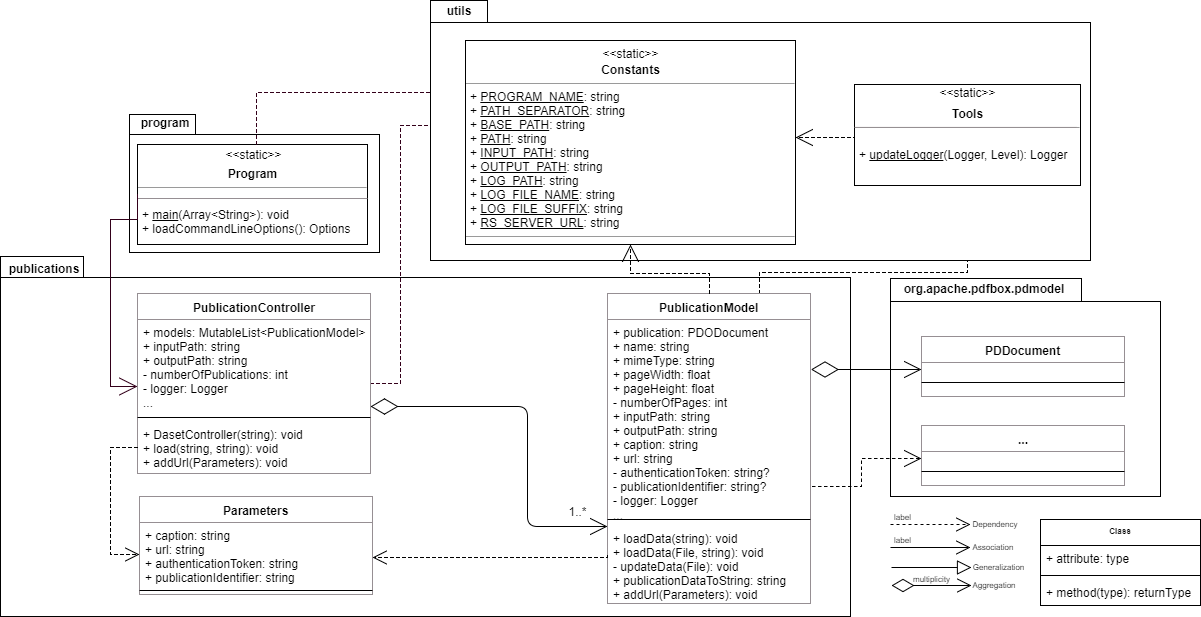
\includegraphics[scale=0.55, angle=90]{figures/classi-2.png}
\caption{Class diagram of \rspdf.}
\label{fig:classi-2}
\end{figure}

\subsection{Installation}

\rspdf comes bundled with \rsserver, eliminating the need for manual installation when deploying the latter. However, if you wish to use \rspdf 
independently, you can simply download the attached \verb|.jar| files from the release section of the repository\footnote{\url{https://github.com/Miccighel/Readersourcing-2.0-RS_PDF}} and place them anywhere on your filesystem.

\subsubsection{Requirements}

\begin{itemize}
\item JDK (Java Development Kit) $==$ 11.0.19;
\end{itemize}

\subsubsection{Commmand Line Interface}

The behavior of \rspdf is configured during its startup phase by \rsserver through a set of special command-line options. For this reason, it is useful to provide a list of all the options that can be used if it is necessary to employ \rspdf in other contexts, modify its implementation, or for any other reason. However, it is designed to work with a default configuration if no options are provided. This list of command-line options is shown in Table~\ref{tab:cli}.

\begin{table}
\centering
\begin{threeparttable}
\begin{tabular}{p{1cm}p{3cm}p{3cm}p{3cm}p{2cm}p{2cm}}
\toprule
\textbf{Short} & \textbf{Long} & \textbf{Description} & \textbf{Values} & \textbf{Required} & \textbf{Depends On} \\
\midrule
\verb|--pIn| & \verb|--pathIn| & Path on the filesystem from which to load the PDF files to be edited. It can be a file or a folder. & String representing a relative path. & No & \verb|--pOut| \\
\midrule
\verb|--pOut| & \verb|--pathOut| & Path on the filesystem in which to save the edited PDF files. It must be a folder. & String representing a relative path. & No & \verb|--pIn| \\
\midrule
\verb|--c| & \verb|--caption| & Caption of the link to add. & Any string. & Yes & No \\
\midrule
\verb|--u| & \verb|--url| & URL to add. & A valid URL. & Yes & No \\
\midrule
\verb|--a| & \verb|--authToken| & Authentication token received from \rsserver. & A valid authentication token received from \rsserver. & No & \verb|--pOut|, \verb|--pIn|, \verb|--pId| \\
\midrule
\verb|--pId| & \verb|--publicationId| & Identifier for a publication present on \rsserver. & A valid publication identifier received from \rsserver. & No & \verb|--pOut|, \verb|--pIn|, \verb|--a| \\
\bottomrule
\end{tabular}
\caption{Command line options of \rspdf.}
\label{tab:cli}
\end{threeparttable}
\end{table}

To provide an execution example, let's assume a scenario where there is a need to edit some files encoded in PDF format with the following prerequisites:

\begin{itemize}
    \item There is a folder containing $n$ files to edit at the path \verb|C:\data|;
    \item The edited files must be saved inside a folder at the path \verb|C:\out|;
    \item The file in JAR format containing the library is called \verb|RS_PDF-v1.0-alpha.jar|;
    \item The JAR file containing \rspdf is located inside the folder at the path \verb|C:\lib|;
    \item The authentication token received from \rsserver is \\
    \verb|eyJhbGciOiJIUzI1NiJ9....XpC9PMXOjtjRd4NBCtB1a4SfBEi6ndgqsE3k_cEI6Wo|;
    \item The publication identifier received from \rsserver is \verb|1|.
\end{itemize}

The execution of \rspdf is started with the following command:

\begin{lstlisting}
java -jar C:\lib\RS_PDF-v1.0-alpha.jar -pIn C:\data -pOut C:\out -a eyJhbGciOiJIUzI1NiJ9....XpC9PMXOjtjRd4NBCtB1a4SfBEi6ndgqsE3k_cEI6Wo -pId 1
\end{lstlisting}

\section{\rsrate}

\label{rs-rate}

\rsrate~\cite{RS-Rate} is an extension designed to function as a client for the Readersourcing 2.0 ecosystem without requiring access to its website. Compatible with both \emph{Google Chrome}\footnote{\url{https://www.google.com/chrome/}} and \emph{Microsoft Edge},\footnote{\url{https://www.microsoft.com/en-us/edge/}} the extension allows users to rate publications directly from their browsers. This eliminates the need to navigate to the main website, streamlining the process of providing ratings for publications.

The primary objective of \rsrate is to provide readers with a way to seamlessly rate a publication with minimal effort—just a few clicks or keystrokes within the Readersourcing 2.0 ecosystem, contributing to a more dynamic online reading experience. \rsrate serves as the initial client of our project, extending beyond the web-based interface available on the main portal.

Looking ahead, our vision includes expanding the compatibility of \rsrate by developing implementations for other major browsers, such as Firefox, Safari, and other popular browsers. Our commitment is to make this rating tool accessible across a broad range of browsers, ensuring users can seamlessly interact with content and provide feedback, regardless of their preferred browser.

\subsection{Implementation and Technology}

\rsrate is an extension for Google Chrome and, consequently, also for Microsoft Edge. These extensions are developed using standard web technologies such as HTML, CSS, and JavaScript. Therefore, they are simple ``collections'' of files packaged in a CRX archive. This particular format is nothing more than a modified version of a ZIP archive with the addition of some special headers exploited by Google Chrome.

As for the JavaScript component, \rsrate does not actually use the ``pure'' language but instead employs jQuery, a library developed with the aim of simplifying the selection, manipulation, management of events, and the animation of DOM elements in HTML pages. It also implements AJAX features. These AJAX features are widely utilized by \rsrate to enhance the user experience during its use.

\subsection{Installation}

\rsrate is freely available on the Google Chrome Web Store. To use it, simply take advantage of the following link and install the currently available version by clicking on the ``Get'' button shown on the store page. We plan to release a Firefox version in the future.
\begin{itemize}
\item \textbf{Google Chrome} version available at: \url{https://chrome.google.com/webstore/detail/readersourcing-20-rsrate/hlkdlngpijhdkbdlhmgeemffaoacjagg?hl=it}
\end{itemize}

\subsection{Usage}

Figure~\ref{fig:ux-1} illustrates a section of a Google Chrome instance with the extension active for a publication. This scenario depicts the typical situation of a reader visiting a publisher's website to access the PDF of a paper they are interested in. The figure also displays the initial page that a reader encounters when interacting with the client. This page serves as a gateway to the login page, as shown in Figure~\ref{fig:login}, or to the sign-up page. From the login page, a reader who has forgotten their password can access the password recovery page (not shown), which closely resembles the login page.

\begin{figure}
\centering
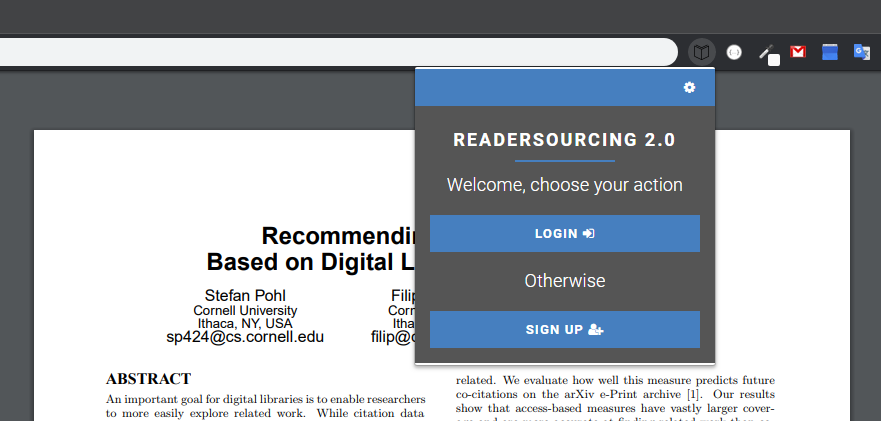
\includegraphics[width=\textwidth]{figures/ux-1.png}
\caption{\rsrate characterized as an extension having a popup action.}
\label{fig:ux-1}
\end{figure}

\begin{figure}
\centering
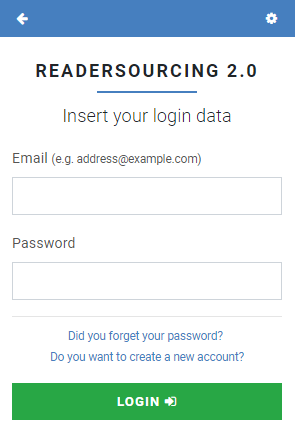
\includegraphics[scale=0.7]{figures/login.png}
\caption{The login page of \rsrate.}
\label{fig:login}
\end{figure}

If a reader has yet to sign up for Readersourcing 2.0, they can navigate from the page shown in Figure~\ref{fig:ux-1} to the one displayed in Figure~\ref{fig:signup} and fill in the sign-up form. Once they complete the standard sign-up and login operations, they will find themselves on the rating page, as shown in Figure~\ref{fig:rating-1}.

\begin{figure}
\centering
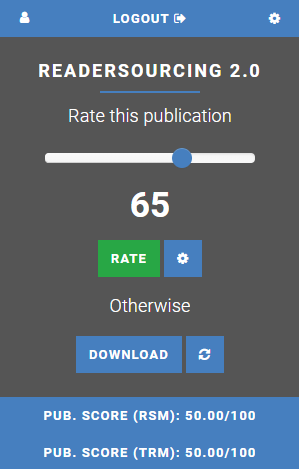
\includegraphics[scale=0.7]{figures/rating-2.PNG}
\caption{The rating page of \rsrate.}
\label{fig:rating-1}
\end{figure}

\begin{figure}
\centering
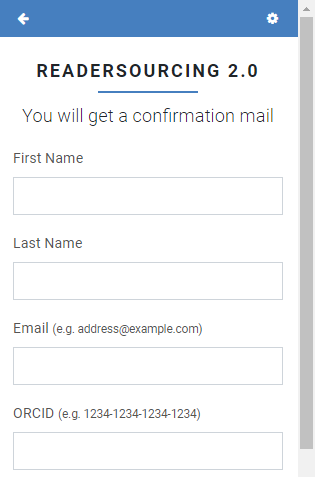
\includegraphics[scale=0.7]{figures/signup.PNG}
\caption{The user registration page of \rsrate.}
\label{fig:signup}
\end{figure}


In the central section of the rating page, a reader can use the slider to choose a rating value in a 0-100 interval. Once they select the desired rating, they only need to click the green \emph{Rate} button, and that's it; with just three clicks and a slide action, they can submit their rating. Furthermore, they can also click the options button and, if preferred, check an option to anonymize the rating they are about to provide. It's important to note that the reader has to be logged in to express an anonymous rating to prevent spamming, which in this case would be a very dangerous phenomenon. When such a rating is processed, the information regarding its reader will not be used, except for preventing the reader from rating the same publication multiple times.

If the reader prefers to provide their rating at a later time instead of immediately rating the publication, they can click the \emph{Save for later} button. This option allows them to take advantage of the editing procedure for publications, which stores a reference (an URL link) inside the PDF file they are viewing. As soon as such the editing procedure is completed (usually just a few seconds), the \emph{Save for later} button transforms into a \emph{Download} button, as shown in Figure~\ref{fig:rating-2}.

\begin{figure}
\centering
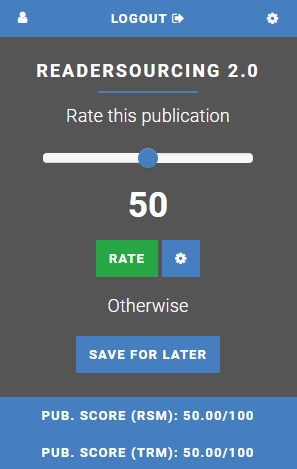
\includegraphics[scale=0.7]{figures/rating.PNG}
\caption{The rating page of \rsrate after a \lq\lq save for later\rq\rq{} request.}
\label{fig:rating-2}
\end{figure}

The reader can finally download the link-annotated publication by clicking on it. Furthermore, they can also use the refresh button (located to the right of the \emph{Download} button) to, as it says, refresh the link-annotated publication. This means that a new copy of the publication file will be downloaded, annotated, and made available to the reader. This feature is useful since a publication could be updated at a later time by its author.

As soon as the link-annotated publication is downloaded, the reader will find a PDF containing a new final page with the URL. In Figure~\ref{fig:reference}, an example of such a link-annotated publication can be seen; in that case, the reader has chosen to open it with their favorite PDF reader.

\begin{figure}
\centering
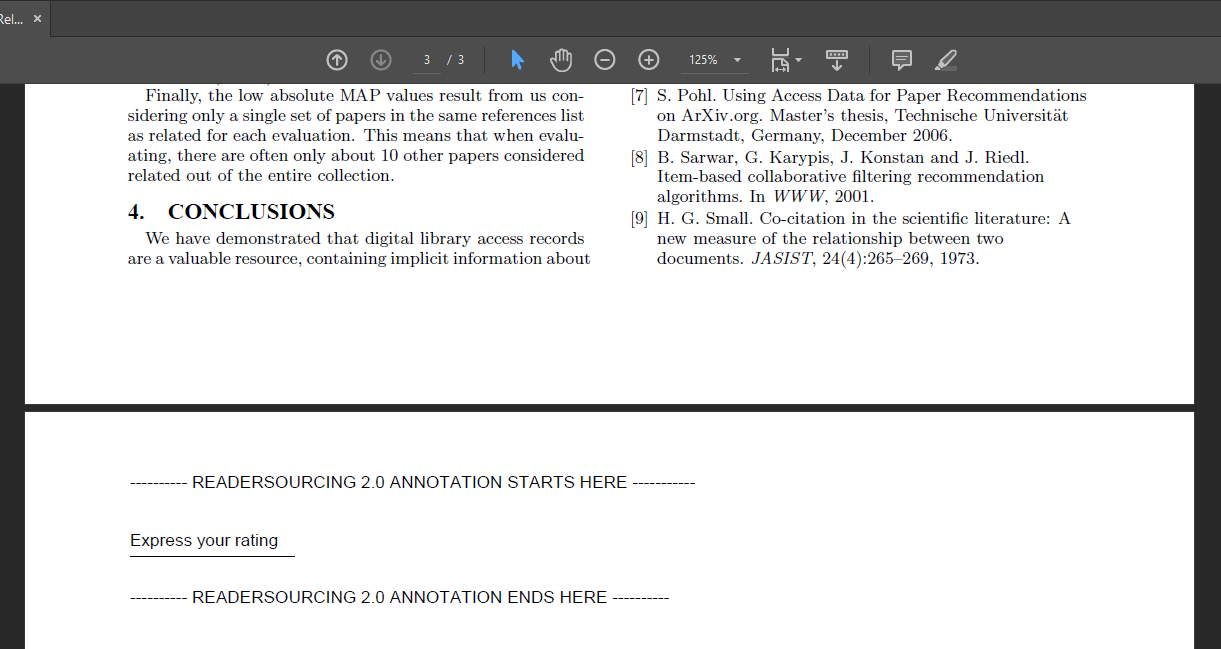
\includegraphics[width=\textwidth]{figures/reference.png}
\caption{A publication link-annotated through \rsrate.}
\label{fig:reference}
\end{figure}

Once the reader clicks on the reference, which is a special link to \rsserver, they will be taken to the server-side application itself. The interface presented allows them to express their rating independently of the browser extension used to store the reference. Therefore, if they send their link-annotated publication to a tablet-like device, for example, they can take advantage of the built-in browser to express their rating. Figure~\ref{fig:browser} shows the interface that the reader sees after clicking on the stored reference. The reader is required to authenticate themselves again as a form of security. Without this step, the stored reference could be used by anyone who gets a copy of the link-annotated publication.

\begin{figure}
\centering
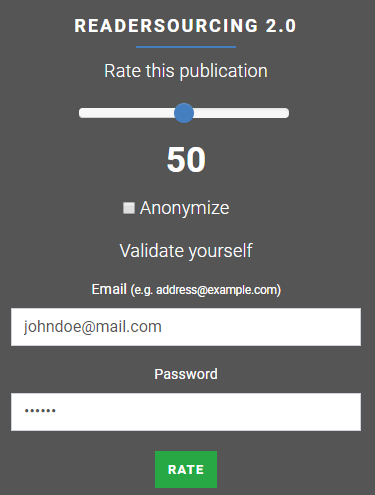
\includegraphics[scale=0.7]{figures/browser.png}
\caption{The server-side interface to rate a publication.}
\label{fig:browser}
\end{figure}

Every time a reader rates a publication, every score is updated according to both RSM and TRM models, and each reader can see the result through \rsrate. In the bottom section of the rating page, the score of the current publication can be seen (one for each model), as shown in Figures~\ref{fig:rating-1} and~\ref{fig:rating-2}. To view their score as a reader (once again, one for each model), a user must click the profile button in the upper right corner. Once they do that, they will see the interface shown in Figure~\ref{fig:profile}. From there, they can also edit their password since that interface acts as a profile page.

\begin{figure}
\centering
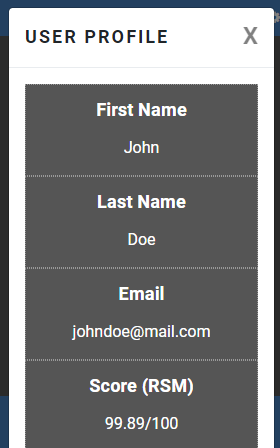
\includegraphics[scale=0.7]{figures/profile.png}
\caption{The profile page of \rsrate.}
\label{fig:profile}
\end{figure}

\section{\rspy}

\label{rs-py}

\rspy \cite{RS-Py} is an additional component of the Readersourcing 2.0 ecosystem, providing a fully working implementation of the models presented by \citet{Soprano2019}. These models are encapsulated by the server-side application of Readersourcing 2.0, as described in Section~\ref{rs-server}. 

Developers with a background in the Python programming language can leverage \rspy to generate and test new simulations of ratings given by readers to a set of publications. They are allowed to alter the internal logic of the models to test new approaches without the need to fork and edit the full implementation of Readersourcing 2.0.

\subsection{Implementation and Technology}

\rspy is a collection of \emph{Jupyter Notebooks}. Jupyter\footnote{\url{https://jupyter.org/}} is a Python-powered\footnote{\url{https://www.python.org/}} open-source web application that allows the creation and sharing of documents containing live code, equations, visualizations, and narrative text. Notebooks can be shared with others and are composed of cells that can be run independently, providing a step-by-step overview of the implemented computations.

\subsection{Installation}

To use \rspy notebooks, it is sufficient to clone its repository\footnote{\url{https://github.com/Miccighel/Readersourcing-2.0-RS_Py}} and place it somewhere on the filesystem. Ensure that the required Python packages are installed by leveraging a distribution such as Anaconda\footnote{\url{https://www.anaconda.com/distribution/}}. If a lightweight installation is preferred, an instance of Python 3.7.3 or higher is needed to install the required packages, such as Jupyter, Pandas, and others.

\subsection{Usage}

\rspy is organized into five main folders on the filesystem:

\begin{itemize}
    \item The \verb|data| folder is used to store the dataset exploited to test the models presented by \citet{Soprano2019}.
    \item The \verb|models| folder is used to store the output of these models.
    \item The \verb|notebooks| folder contains Jupyter notebooks used to generate new datasets and implement the models presented by \citet{Soprano2019}.
    \item The \verb|scripts| folder contains implementations of the Jupyter notebooks as pure Python scripts.
    \item The \verb|src| folder contains a Python script which converts Jupyter notebooks into pure Python scripts.
\end{itemize}

Within the \verb|notebooks| folder, three Jupyter notebooks are available:

\begin{itemize}
    \item \verb|Readersourcing.ipynb| provides an implementation of the RSM model presented by \citet{Soprano2019}.
    \item \verb|TrueReview.ipynb| offers an implementation of the TRM model.
    \item The \verb|Seeder.ipynb| notebook allows the generation of new datasets, which will be stored inside the \verb|data| folder.
\end{itemize}

Inside the \verb|src| folder, the \verb|Convert.py| script enables the conversion of notebooks into Python scripts, and these are then stored inside the \verb|scripts| folder.

The behavior of \verb|Seeder.ipynb| and \verb|Readersourcing.ipynb| notebooks can be customized by modifying the parameter settings found in the initial rows of both notebooks. Table~\ref{tab:seeder-notebook} outlines the parameters available for the former, while Table~\ref{tab:readersourcing-notebook} presents the parameters for the latter.

To run and use the Jupyter notebooks, navigate to the main directory of \rspy using a command-line prompt (you should see folders such as \verb|data|, \verb|models|, \verb|notebooks|, etc.) and type \verb|jupyter notebook|.\footnote{\url{https://jupyter.readthedocs.io/en/latest/running.html\#running}} This command will start the Jupyter server, and you can access the \emph{Notebook Dashboard} in your browser at the web application's URL (typically, \verb|http://localhost:8888|).

\begin{table}
\centering
\begin{tabular}{p{3cm}p{7cm}p{3cm}}
\toprule
\textbf{Parameter} & \textbf{Description} & \textbf{Values} \\
\midrule
\verb|dataset_name| & Name of the dataset to simulate & String \\
\verb|papers_number| & Number of papers to simulate & Positive integer \\
\verb|readers_number| & Number of readers to simulate & Positive integer \\
\verb|authors_number| & Number of authors to simulate & Positive integer \\
\verb|months_number| & Number of months of activity to simulate & Positive integer \\
\verb|paper_frequencies| & Amount of papers rated by each reader group & Array of positive integers \\
\verb|readers_percent| & Percentage of readers to assign to a single group & Positive integer\\
\bottomrule
\end{tabular}
\caption{Parameters available for the Seeder Jupyter notebook.}
\label{tab:seeder-notebook}
\end{table}

\begin{table}
\centering
\begin{tabular}{p{5cm}p{5.5cm}p{2.5cm}}
\toprule
\textbf{Parameter} & \textbf{Description} & \textbf{Values} \\
\midrule
\verb|dataset_name| & Name of the dataset to simulate & String \\
\verb|day_serialization| & Activate serialization of data on a per-day basis & True, False \\
\verb|day_serialization_threshold| & Serialize data every X days & Positive integer \\
\verb|days_number| & Amount of days simulated in the input dataset & Positive integer \\
\bottomrule
\end{tabular}
\caption{Parameters available for the Readersourcing Jupyter notebook.}
\label{tab:readersourcing-notebook}
\end{table}

\section{Overview}

\label{overview}

An overview of Readersourcing 2.0 capabilities is shown in Figure~\ref{fig:scenario}. Let us suppose that there are four readers using \rsrate to rate a publication, \verb|P1|, namely \verb|RD1|, \verb|RD2|, \verb|RD3|, and \verb|RD4|. Both \verb|RD1|, \verb|RD2|, and \verb|RD3| utilize the \emph{Save for later} functionality of \rsrate to express their ratings at a later time. By doing this, they receive a link-annotated version of \verb|P1|, namely \verb|P1+Link|. 

After some time, \verb|RD1| chooses to open \verb|P1+Link| with his favorite PDF reader. \verb|RD2|, instead, sends it to his tablet, while \verb|RD3| simply opens it with his instance of Google Chrome. When they click on the URL added by \rsserver, they are taken to the special page provided by \rsserver where they provide their ratings. On the contrary, \verb|RD4| simply chooses to give his rating as soon as he finishes reading \verb|P1| directly through the \rsrate interface.

\begin{figure}
\centering
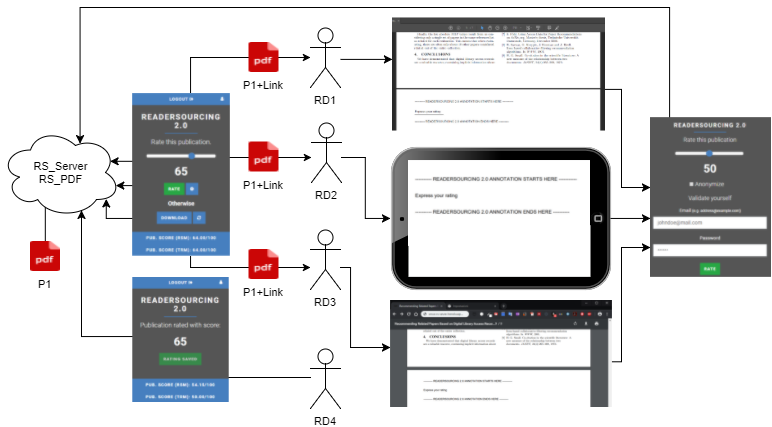
\includegraphics[width=\textwidth]{figures/scenario.png}
\caption{Readers' interaction modalities with the Readersourcing 2.0 ecosystem.}\label{fig:scenario}
\end{figure}

\newpage

\nocite{*}
\printbibliography[heading=bibintoc]

\end{document}
